% ====================================================================
% VİZE RAPOR ŞABLONU – Türk Masalları Derlemesi Web Sayfası
% --------------------------------------------------------------------
% DERLEME: Overleaf'te Menu > Compiler > XeLaTeX (pdfLaTeX de çalışır).
%
% KURALLAR (şablonu kullanmadan önce okuyun):
%  1. Bölüm başlıklarını SİLMEYİN ve sırasını DEĞİŞTİRMEYİN.
%  2. [KÖŞELİ PARANTEZ] içindeki ve gri renkli açıklama metinlerini
%     kendi bilgilerinizle değiştirin; açıklama metinlerini silin.
%  3. MEBİS'e YALNIZCA bu raporun PDF'ini yükleyin.
%     ZIP ve HTML dosyası YÜKLEMEYİN. Tüm kontroller GitHub'dan yapılır.
%  4. Kapaktaki GitHub ve YouTube bağlantıları doğru ve tıklanabilir
%     olmalıdır. Teslimden önce PDF'teki bağlantılara tıklayıp deneyin.
%  5. Haftalık katkı tablosundaki görseller için resim dosyalarını
%     (hafta1.png, hafta2.png, ...) Overleaf projesine yükleyin.
%     Dosya adlarında boşluk ve Türkçe karakter kullanmayın.
%     Resim yoksa tabloda "görsel ekleyin" kutusu görünür.
%  6. Yapay zekâ kullandıysanız Bölüm 5'i doldurun.
% ====================================================================
\documentclass[12pt,a4paper]{article}

\usepackage{iftex}
\ifPDFTeX
  \usepackage[T1]{fontenc}
  \usepackage[utf8]{inputenc}
\else
  \usepackage{fontspec}
\fi
\usepackage[turkish]{babel}
\usepackage[margin=2.4cm]{geometry}
\usepackage{setspace}
\usepackage{graphicx}
\usepackage{float}
\usepackage{booktabs}
\usepackage{longtable}
\usepackage{array}
\usepackage{colortbl}
\usepackage{xcolor}
\usepackage{enumitem}
\usepackage{listings}
\usepackage{amssymb}
\usepackage{caption}
\usepackage{fancyhdr}
\usepackage{hyperref}

\onehalfspacing
\setlength{\parindent}{0pt}
\setlength{\parskip}{6pt}
\setlist{itemsep=2pt, topsep=4pt}
\hypersetup{colorlinks=true, linkcolor=blue!50!black, urlcolor=blue!50!black}

\definecolor{ana}{HTML}{14325C}
\definecolor{acik}{HTML}{EEF2F8}

\lstset{basicstyle=\ttfamily\small, backgroundcolor=\color{acik},
  frame=single, rulecolor=\color{ana}, breaklines=true,
  columns=fullflexible, keepspaces=true, showstringspaces=false}

\pagestyle{fancy}
\fancyhf{}
\fancyhead[L]{Masal Ormanı}
\fancyhead[R]{Vize Raporu}
\fancyfoot[C]{\thepage}

% ---------- Yardımcı komutlar ----------
% Gri açıklama metni (silinecek yönergeler için)
\newcommand{\aciklama}[1]{{\color{gray}\itshape (#1)}}

% Haftalık tablo görseli: dosya yoksa "görsel ekleyin" kutusu çıkar
\newcommand{\haftagorsel}[1]{%
  \IfFileExists{#1}{%
    \includegraphics[width=\linewidth,height=2.8cm,keepaspectratio]{#1}%
  }{%
    \fbox{\parbox[c][2.6cm][c]{\dimexpr\linewidth-2\fboxsep-2\fboxrule\relax}{%
      \centering\small\color{gray} Ekran görüntüsü / görsel ekleyin\\ \texttt{#1}}}%
  }%
}
% Haftalık katılım kutuları (işaretlemek için $\square$ yerine $\boxtimes$ yazın)
\newcommand{\katilimkutulari}{\par\vspace{3pt}\small $\square$ Ders içinde katılım sergiledim\par $\square$ Telafi yaptım}

% Ek görsel: dosya yoksa hiçbir şey göstermez
\newcommand{\haftaek}[1]{%
  \IfFileExists{#1}{\\[4pt]\includegraphics[width=\linewidth,height=4.2cm,keepaspectratio]{#1}}{}%
}

% ---------- Kapak bilgileri ----------
\newcommand{\universite}{İstanbul Medipol Üniversitesi}
\newcommand{\dersadi}{Programlamaya Giriş}
\newcommand{\hocaadi}{Meral Şentürk}
\newcommand{\ogrenciadi}{İrem Başak Tunç}
\newcommand{\ogrencino}{86220033}
\newcommand{\projeadi}{Masal Ormanı}
% Bağlantıları tam adres olarak yazın (https:// ile başlayarak)
\newcommand{\githublink}{\url{https://github.com/Irembasak-tnc/Masal-Orman-}}
\newcommand{\youtubelink}{\url{https://youtu.be/JN4zs9tCGRk}}

\begin{document}

% ====================================================================
% KAPAK
% ====================================================================
\begin{titlepage}
\centering
\vspace*{1cm}
{\large \universite \par}
\vspace{1.8cm}
{\Huge\bfseries\color{ana} \projeadi \par}
\vspace{0.4cm}
{\Large Türk Masallarının Dijital Dünyası \par}
{\large Vize Raporu \par}
\vspace{1.8cm}
{\large \textbf{Ders:} \dersadi \par}
{\large \textbf{Öğretim Üyesi:} \hocaadi \par}
\vspace{1.2cm}
{\large \textbf{Hazırlayan:} \ogrenciadi \par}
{\large \textbf{Öğrenci No:} \ogrencino \par}
\vspace{1.8cm}
\fbox{\parbox{0.88\linewidth}{\centering\vspace{6pt}
{\large\bfseries Proje Bağlantıları}\\[8pt]
\textbf{GitHub deposu:}\\ \githublink \\[8pt]
\textbf{YouTube sunum videosu:}\\ \youtubelink
\vspace{6pt}}}
\vfill
{\large \today \par}
\end{titlepage}

\tableofcontents
\newpage

% ====================================================================
\section{Giriş}
% ====================================================================
Bu projenin amacı, Türk masallarını dijital bir ortamda bir araya getirerek kullanıcıların bu masallara kolayca ulaşmasını sağlamaktır. Bu amaçla “Masal Ormanı” adını verdiğim, fantastik ve gizemli bir tasarıma sahip web sitesi oluşturdum. Sitede Keloğlan ve Padişah, Zümrüdüanka Kuşu ve İğci Baba gibi toplam sekiz Türk masalına yer verdim. Çünkü sitenin atmosferiyle uyucağını düşündüm.Her masal için görsel ve başlık içeren ayrı kartlar hazırladım. Projeyi tek bir HTML dosyası içerisinde oluşturdum ve tasarımını HTML dosyasına eklediğim CSS kodlarıyla düzenledim. JavaScript kullanarak masalların açılıp kapanmasını sağladım. Böylece kullanıcıların masalları kolayca seçip okuyabileceği, farklı ekran boyutlarında kullanılabilen bir web sitesi hazırladım.



\subsection{Proje Özeti}
Masal Ormanı, Türk masallarını dijital ortamda tanıtmak amacıyla hazırlanmış, fantastik temalı ve etkileşimli bir web sitesidir. Projede Keloğlan ve Padişah, Ağlayan Nar ile Gülen Ayva, Zümrüdüanka Kuşu, Billur Köşk, Helvacı Güzeli, Tasa Kuşu, İğci Baba ve Nardaniye Hanım olmak üzere sekiz Türk masalına yer verilmiştir. Kullanıcılar masal kartları aracılığıyla istedikleri masalı seçerek içeriğini okuyabilmektedir. Web sitesi HTML, CSS ve JavaScript kullanılarak geliştirilmiştir.

\subsection{Gereksinimlerin Karşılanması}
\begin{center}
\rowcolors{2}{acik}{white}
\begin{tabular}{@{}p{8.2cm}c@{}}
\toprule
\rowcolor{ana}\textcolor{white}{\textbf{Gereksinim}} & \textcolor{white}{\textbf{Durum}} \\
\midrule
Masal sayısı 8--12 arasında ([8] masal)          & $\boxtimes$ \\
Tek HTML dosyası                                 & $\boxtimes$ \\
Stil kodları içsel (\texttt{<style>} içinde)     & $\boxtimes$ \\
Betik kodları içsel (\texttt{<script>} içinde)   & $\boxtimes$ \\
İnternetsiz açılıp çalışıyor                     & $\boxtimes$ \\
JavaScript sayfada anlamlı bir işlev görüyor     & $\boxtimes$ \\
Masal metinleri kendi cümlelerimle yazıldı       & $\boxtimes$ \\
Sayfa telefonda da düzgün görünüyor              & $\boxtimes$ \\
\bottomrule
\end{tabular}
\end{center}

% ====================================================================
\section{Masalların Seçimi}
% ====================================================================


\begin{longtable}{@{}cp{4cm}p{3cm}p{5.4cm}@{}}
\toprule
\textbf{No} & \textbf{Masal} & \textbf{Tür} & \textbf{Seçilme nedeni} \\
\midrule
\endhead
1 & Keloğlan ve Padişah & Halk masalı & Keloğlan karakterinin zekâsını ve iyiliğini konu alması. \\
2 & Ağlayan Nar ile Gülen Ayva & Olağanüstü masal & Fantastik unsurlar ve farklı karakterler içermesi. \\
3 & Zümrüdüanka Kuşu & Olağanüstü masal & Efsanevi kuş ve macera temasını işlemesi. \\
4 & Billur Köşk & Halk masalı & Geleneksel anlatımı ve masalsı atmosferiyle dikkat çekmesi. \\
5 & Helvacı Güzeli & Halk masalı & Cesaret, mücadele ve yeniden kavuşma temalarını içermesi. \\
6 & Tasa Kuşu & Halk masalı & Kaygı, mutluluk ve hayatın değerini anlatması. \\
7 & İğci Baba & Halk masalı & Zekâ ve yardımlaşma temalarını işlemesi. \\
8 & Nardaniye Hanım & Halk masalı & Kıskançlık, zorluklar ve iyiliğin karşılığını konu alması. \\
\bottomrule
\end{longtable}

% ====================================================================
\section{Tasarım Kararları}
% ====================================================================
Masal Ormanı web sitesinin tasarımını, Türk masallarının fantastik ve gizemli atmosferini yansıtacak şekilde kendim oluşturdum. Arka planda koyu orman yeşili tonlarını kullanarak masal dünyasına uygun bir görünüm elde etmeyi amaçladım. Altın ve parşömen tonlarını ise başlıklarda, yazılarda ve kart detaylarında kullanarak tasarımın bütünlüğünü sağladım.

Masalların kolay bulunabilmesi için her masala ayrı bir kart hazırladım. Kartlarda masalın görseli ve başlığı var. Kullanıcıların ilgilendikleri masalı seçip rahatça okuyabilmeleri için açılır masal alanları oluşturdum. Yazıların okunabilir olmasına, görsellerin içerikle uyum sağlamasına ve sayfanın farklı ekran boyutlarında düzgün görünmesine dikkat ettim. bunu yazıcam bu sekilde

\subsection{Konuya Uygunluk}
Masal Ormanı web sitesi, Türk masallarının fantastik ve gizemli dünyasını yansıtacak şekilde tasarlanmıştır. Koyu orman tonları ve gece mavisi, masalların büyülü atmosferini oluştururken krem ve altın renkleri tasarıma sıcaklık katmaktadır. Kullanılan masal görselleri, hikâyelerin konusunu destekleyerek ziyaretçilerin ilgisini çekmeyi amaçlamaktadır. Sade ve anlaşılır sayfa düzeni sayesinde kullanıcıların masalları rahatça okuyabilmesi hedeflenmiştir.

\subsection{Masal Ormanı web sitesi, Türk masallarının fantastik ve gizemli dünyasını yansıtacak şekilde tasarlanmıştır. Koyu orman yeşili ve altın tonları, büyülü orman atmosferini oluştururken krem rengi metinler okunabilirliği artırmaktadır. Masal görselleri hikâyelerin konusunu desteklemekte, sade sayfa düzeni ise kullanıcıların masalları rahatça okuyabilmesini sağlamaktadır.}
\begin{center}
\rowcolors{2}{acik}{white}
\begin{tabular}{@{}llp{6.4cm}@{}}
\toprule
\rowcolor{ana}\textcolor{white}{\textbf{Ad}} & \textcolor{white}{\textbf{Kod}} & \textcolor{white}{\textbf{Nerede / neden kullandınız?}} \\
\midrule
Koyu orman yeşili & \texttt{\#10271F} & Sayfanın ana arka planında kullanılmıştır. \\
Açık krem & \texttt{\#F3E8D0} & Metinlerde okunabilirliği artırmak için kullanılmıştır. \\
Altın sarısı & \texttt{\#D9B76E} & Başlıklarda, butonlarda ve kenarlıklarda kullanılmıştır. \\
Georgia & -- & Başlık ve metinlerde masalsı ve klasik bir görünüm oluşturmak için seçilmiştir. \\
\bottomrule
\end{tabular}
\end{center}

\subsection{Okunabilirlik, Gezinme ve Duyarlı Tasarım}
\begin{itemize}
  \item \textbf{Okunabilirlik:} Metinlerde açık krem rengi kullanılmış, koyu yeşil arka plan ile yazılar arasında belirgin bir karşıtlık oluşturulmuştur. Georgia yazı tipi tercih edilerek masalsı bir görünüm sağlanmıştır.

  \item \textbf{Gezinme:} Kullanıcılar ana sayfada yer alan masal kartlarını inceleyerek okumak istedikleri masalı seçebilmektedir. Kartlara tıklanınca ilgili masalın içeriği açılmakta, kapatma seçeneğiyle ana sayfaya dönülebilmektedir.

  \item \textbf{Duyarlı tasarım:} Sayfa, farklı ekran boyutlarında kullanılabilecek şekilde düzenlenmiştir. Masal kartları ve içerik alanları ekran genişliğine göre görüntülenmektedir.

  \item \textbf{Tutarlılık:} Sayfa genelinde koyu yeşil, krem ve altın renkleri kullanılmıştır. Başlıklar, kartlar, butonlar ve boşluklar arasında görsel bütünlük sağlanmıştır.
\end{itemize}
\subsection{Ekran Görüntüleri}
\begin{figure}[H]

\centering

\makebox[\textwidth][c]{\scalebox{0.17}{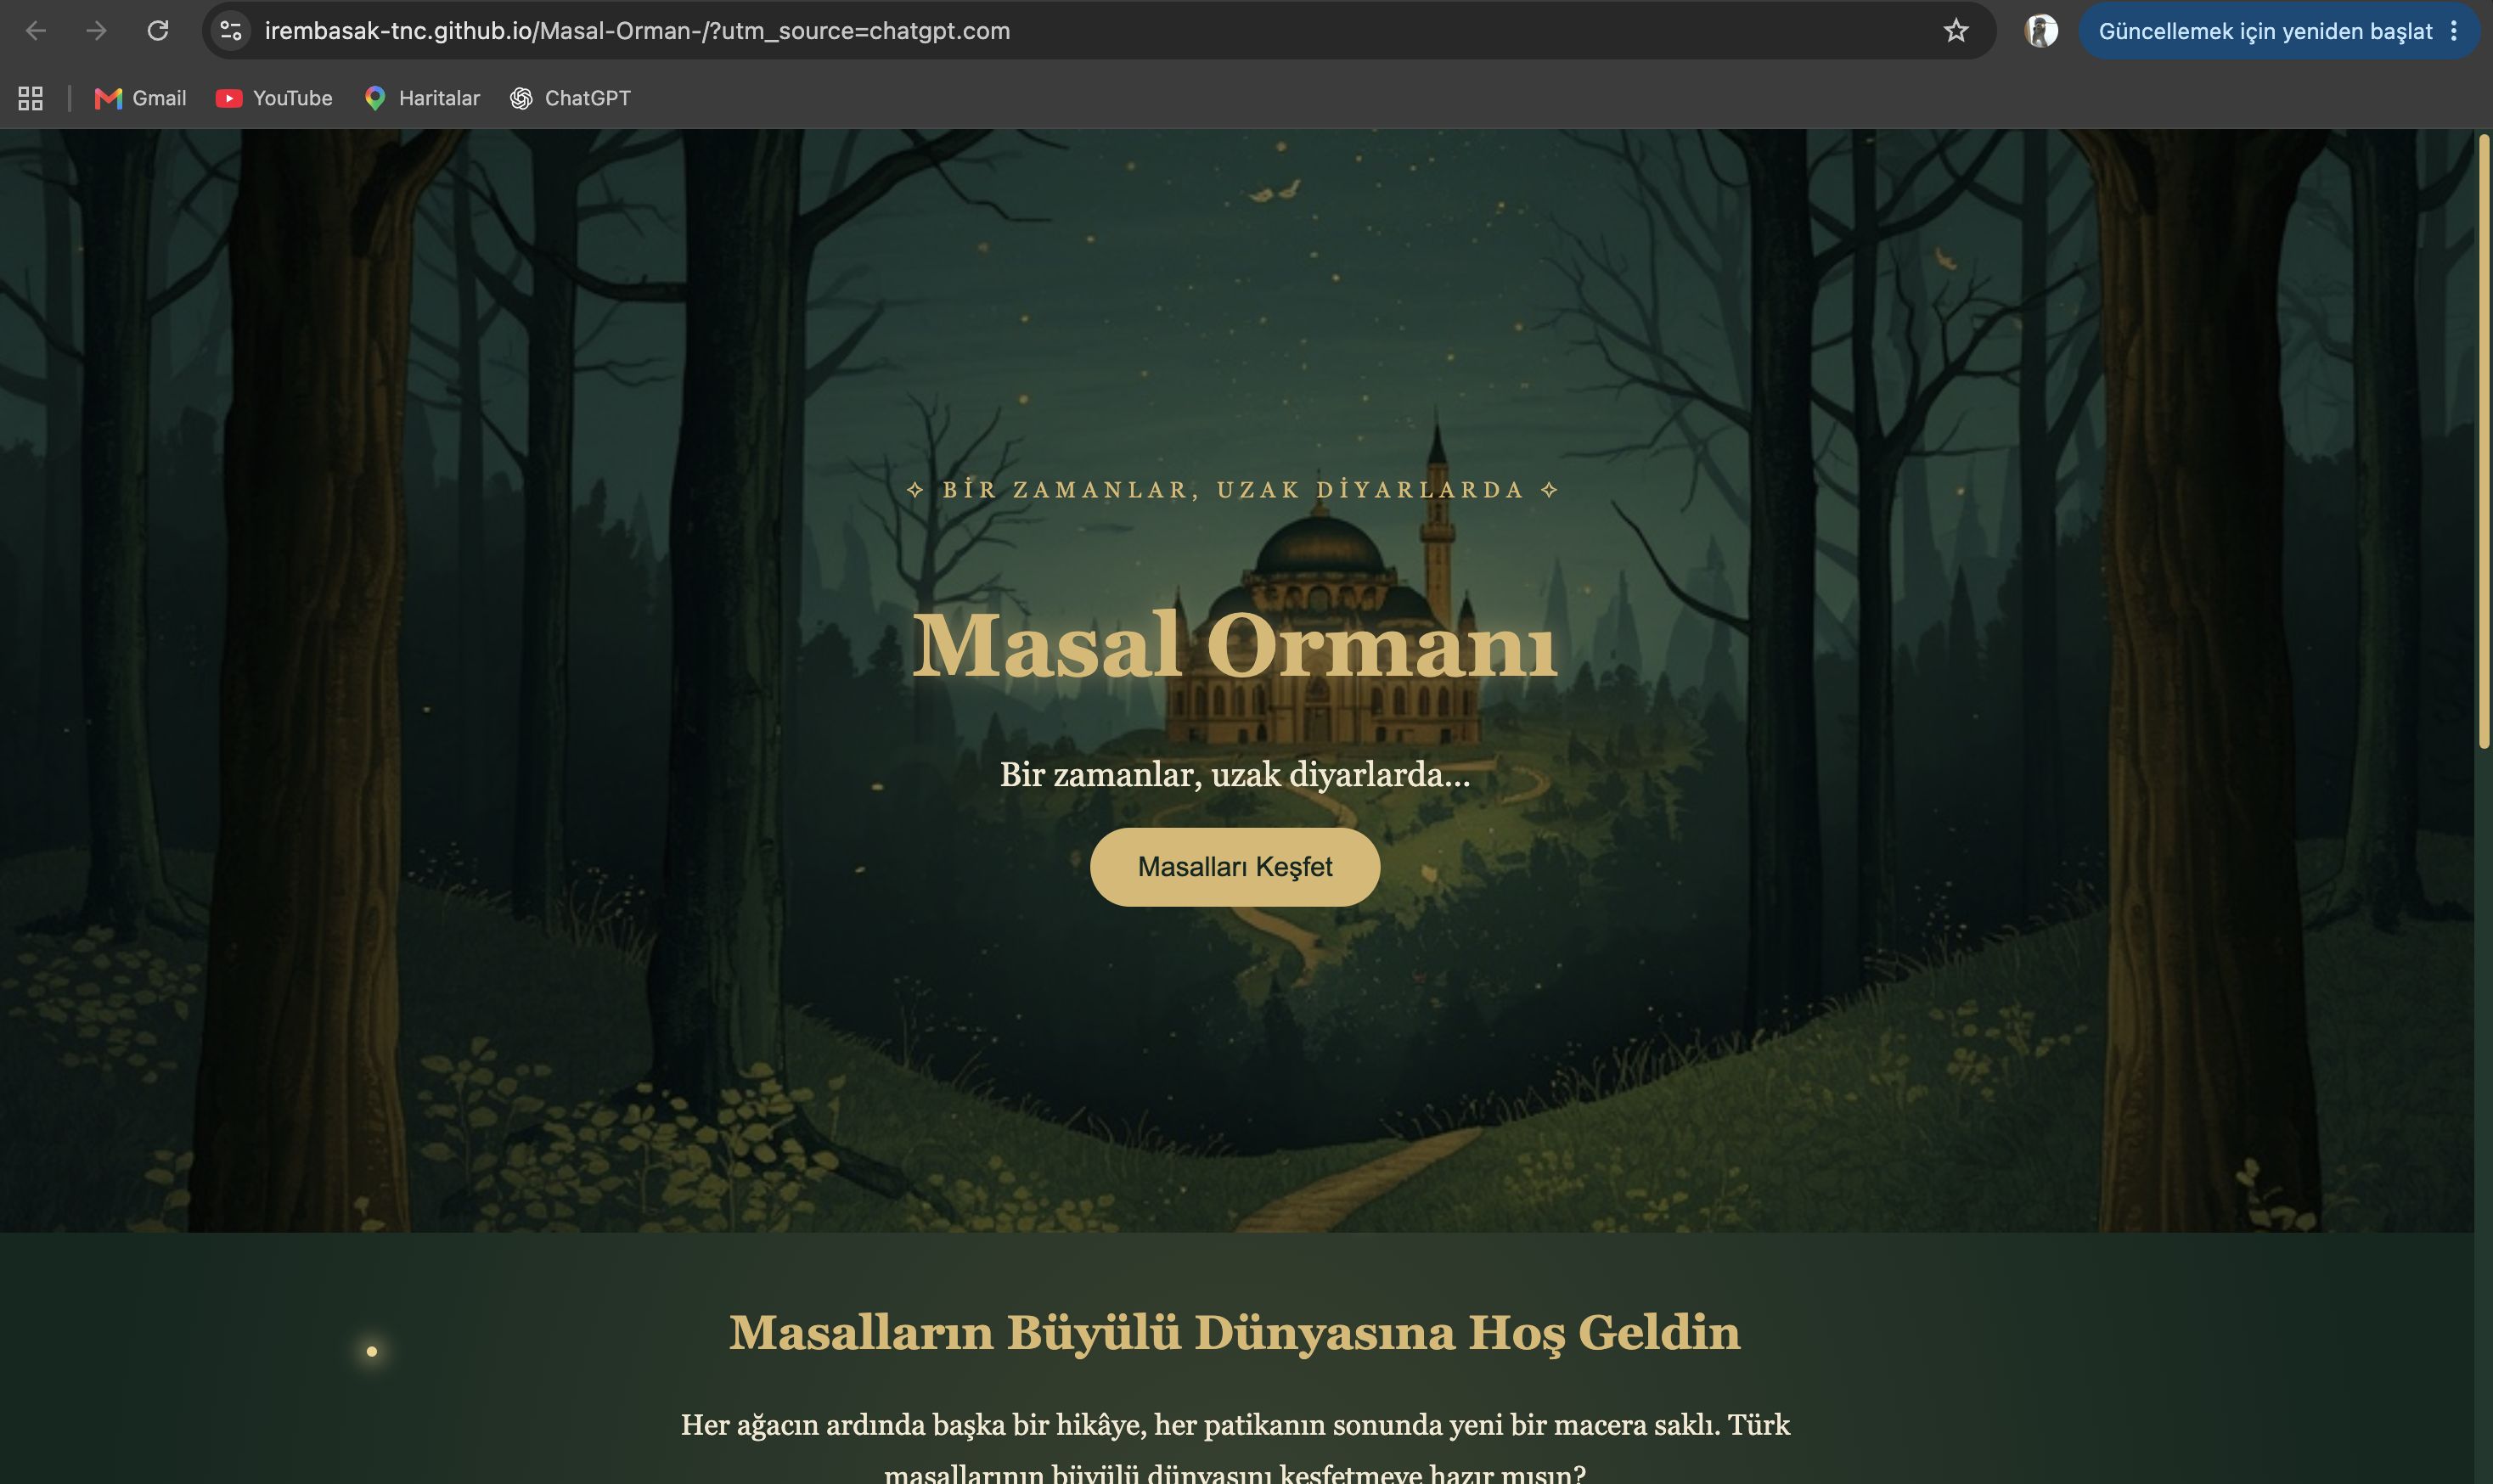
\includegraphics{ekran-masaustu.png}}\hspace{0.5cm}\scalebox{0.17}{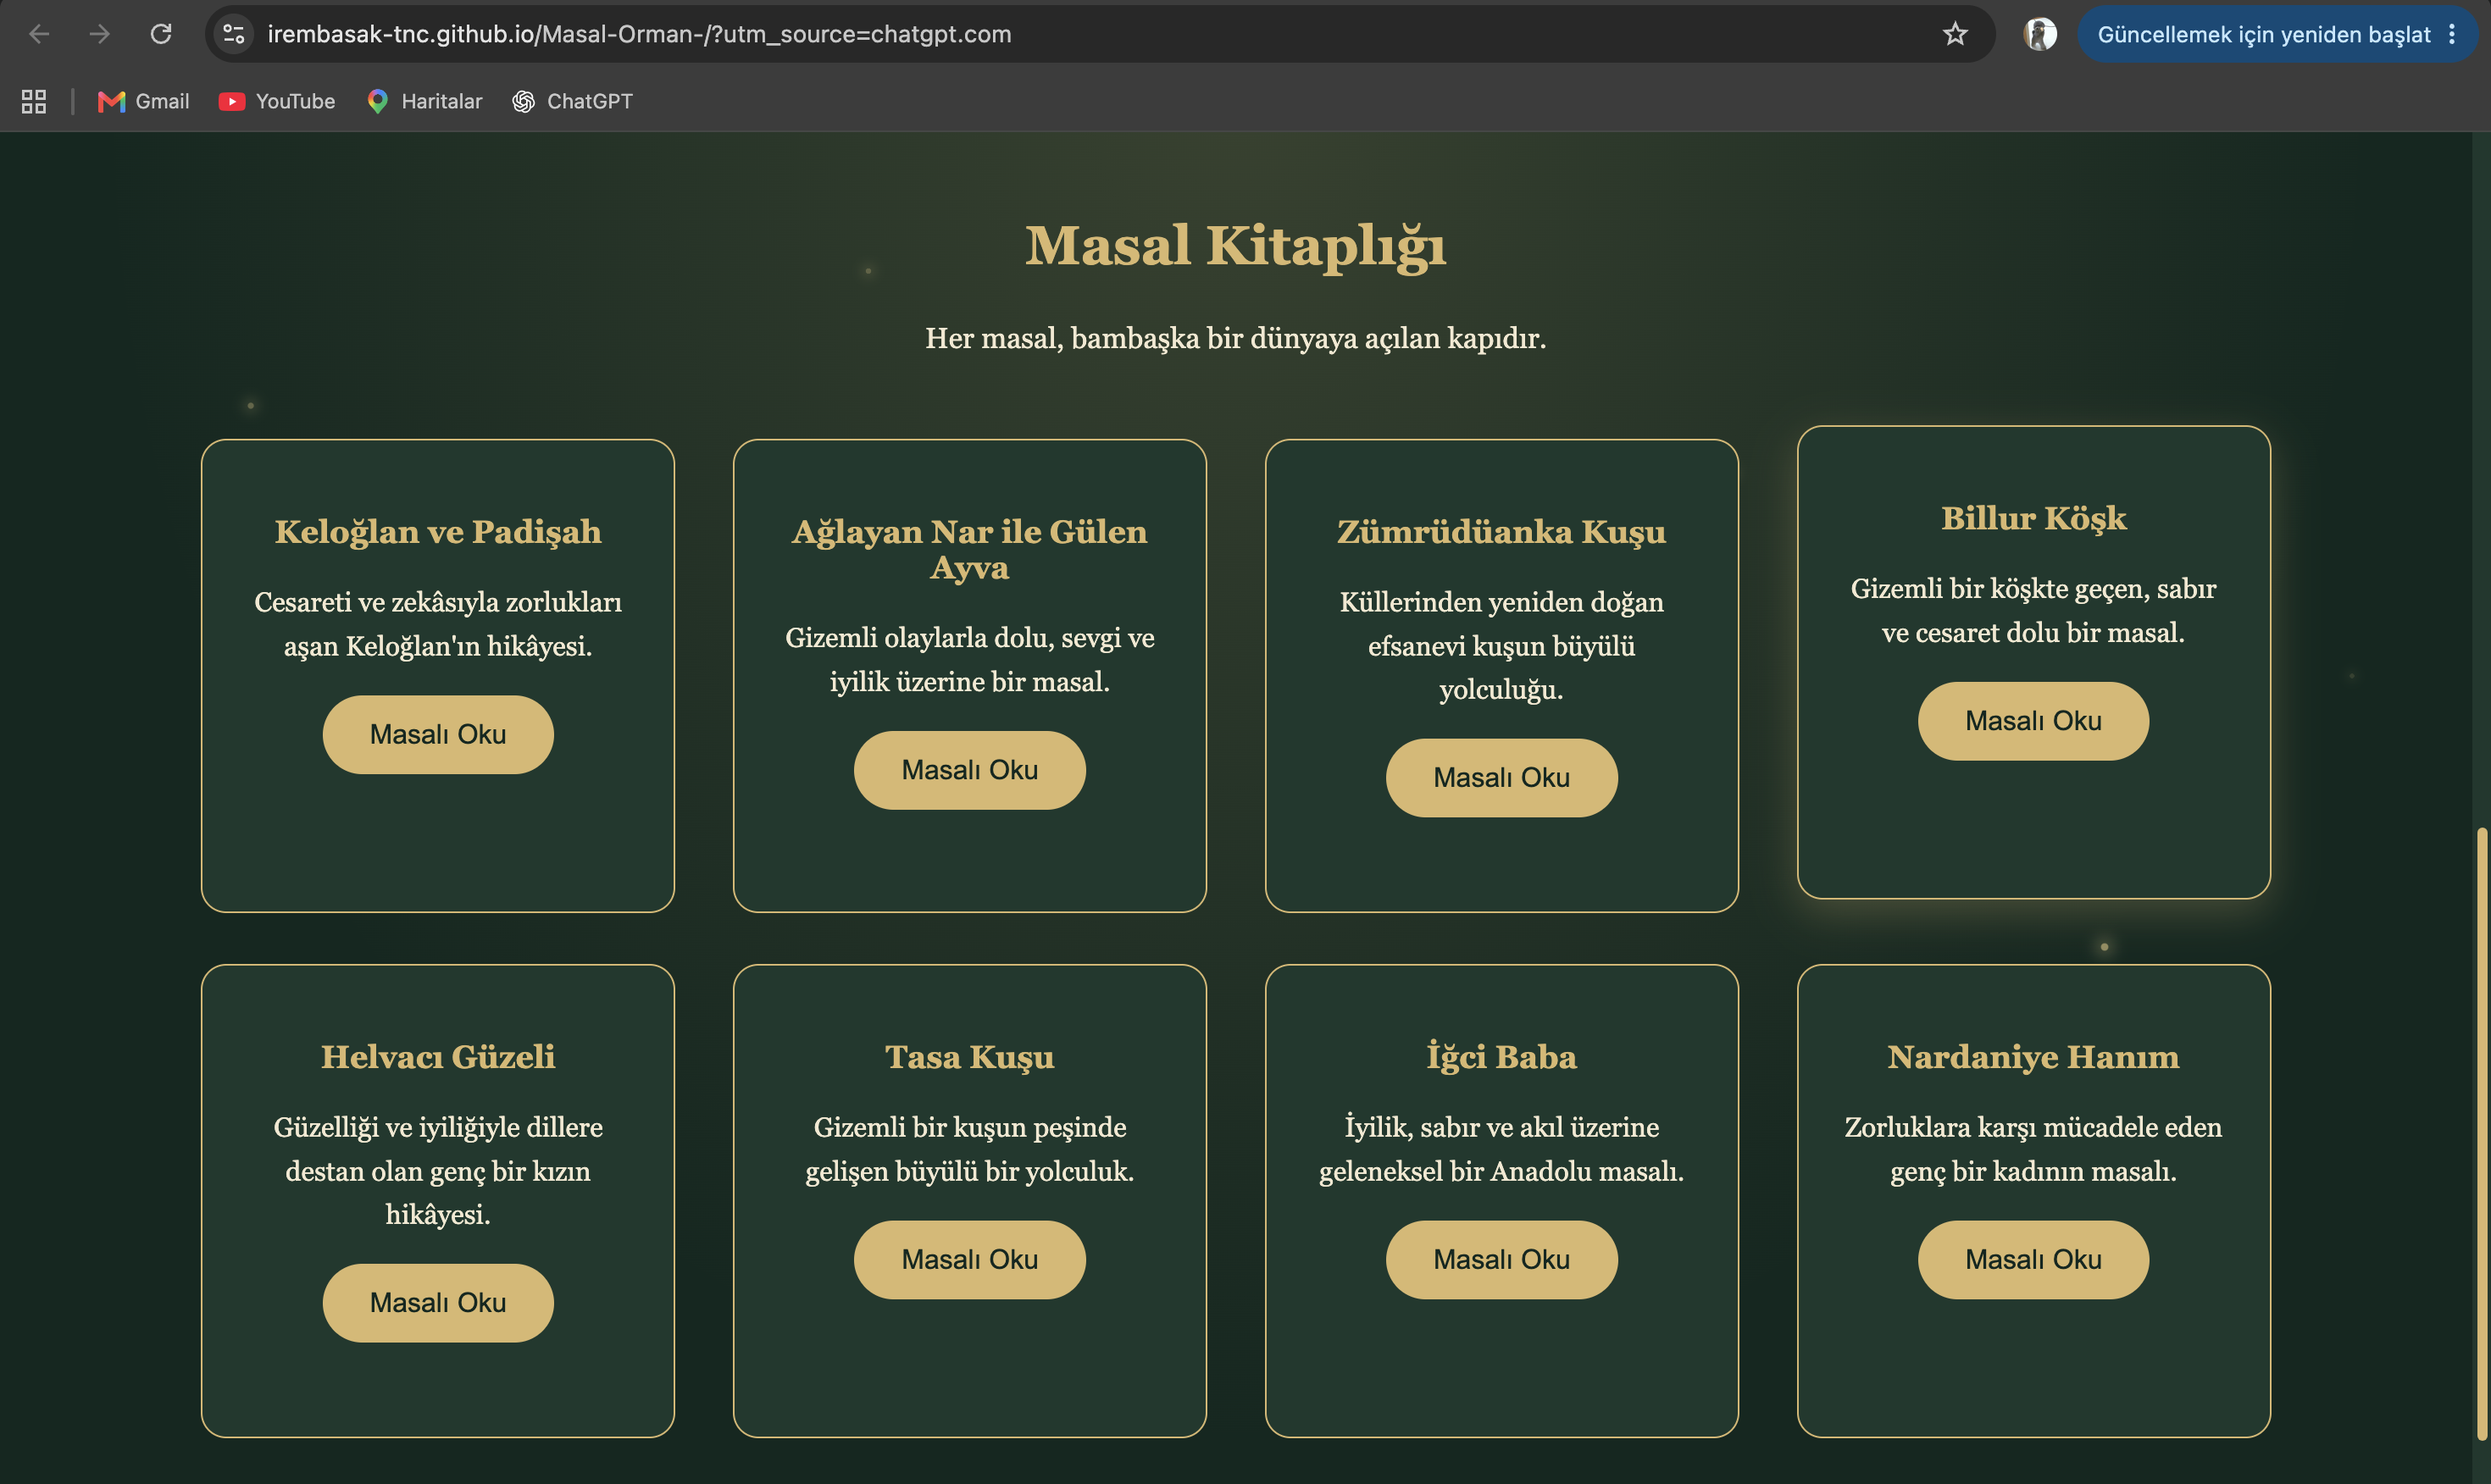
\includegraphics{masal-kartlari.png}}}

\caption{Bilgisayar görünümü ve masal kartları}

\end{figure}
 
 \begin{figure}[H]

\centering

\makebox[\textwidth][c]{\scalebox{0.17}{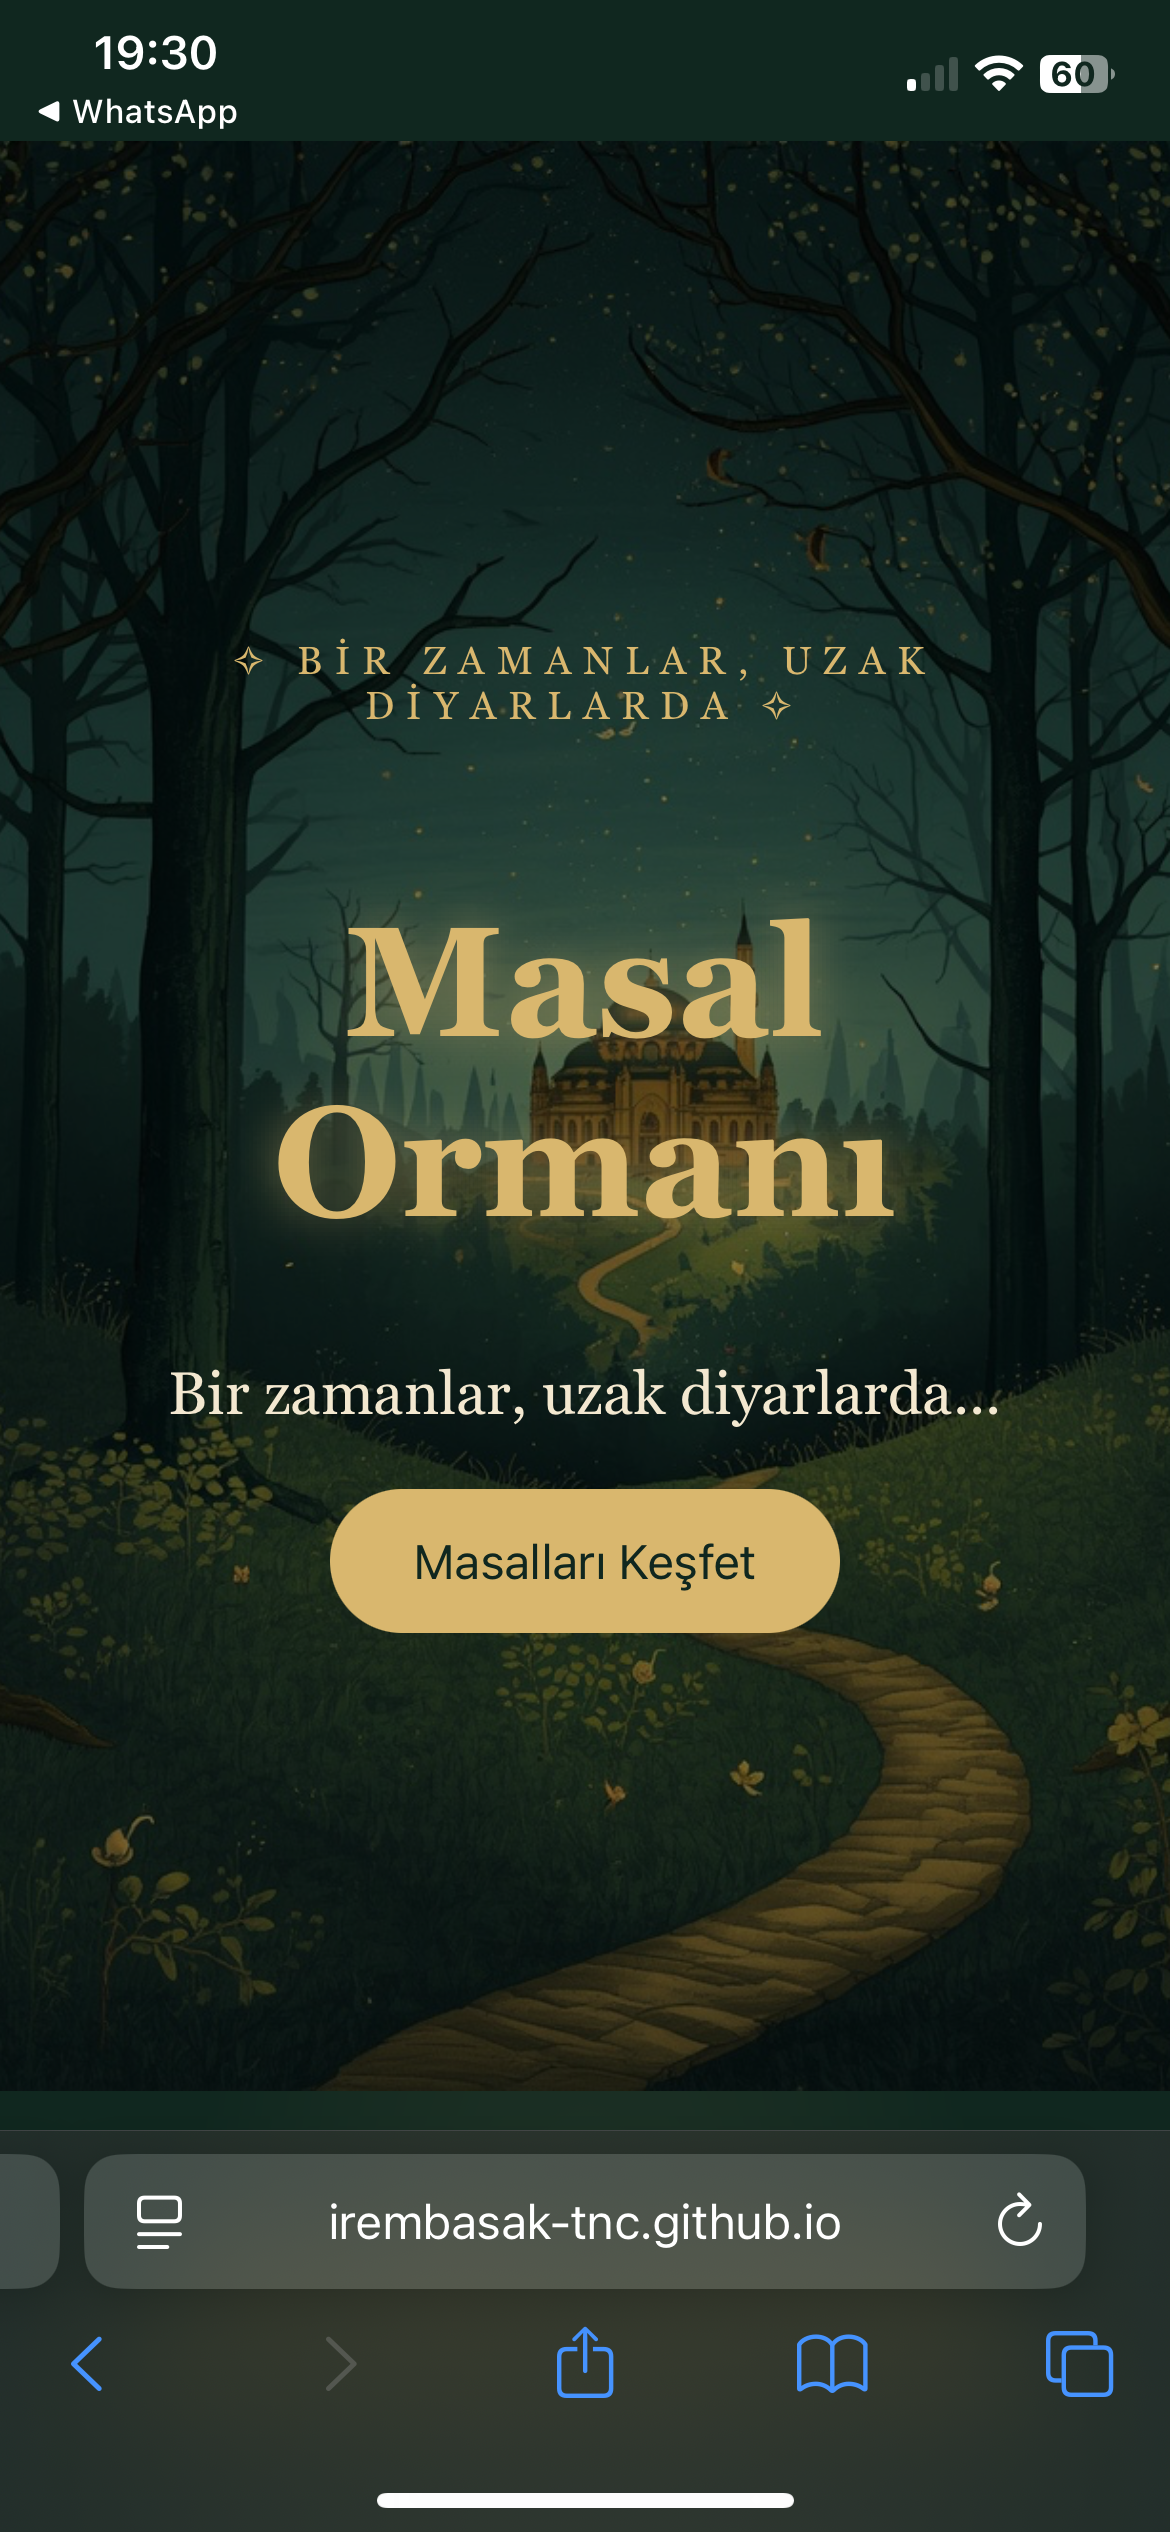
\includegraphics{ekran-mobil.png}}\hspace{0.5cm}\scalebox{0.17}{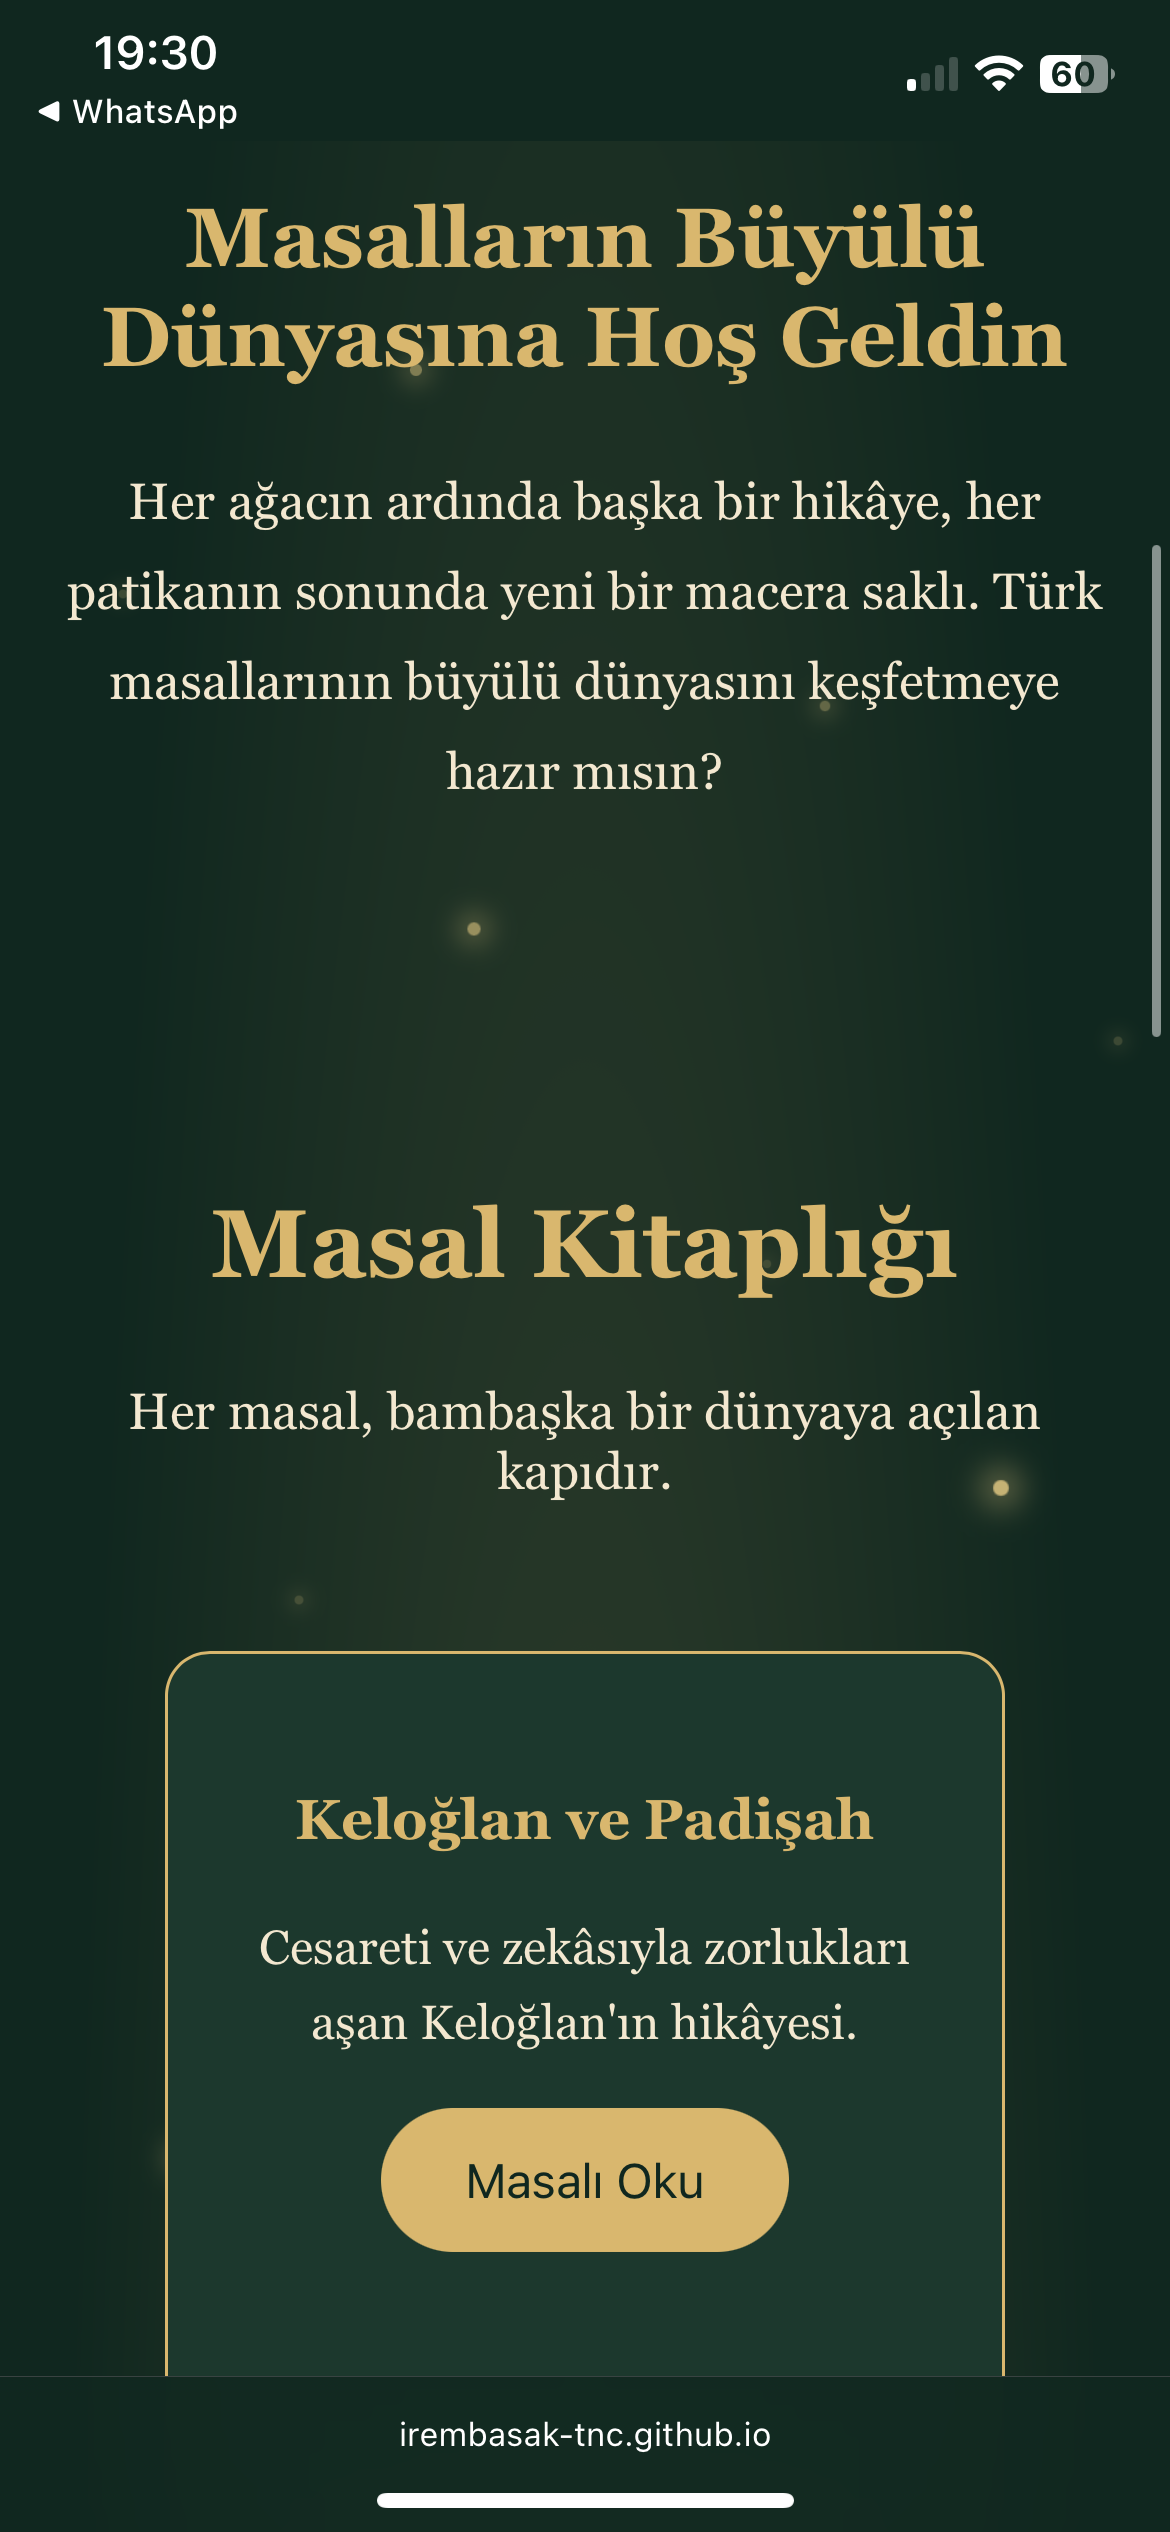
\includegraphics{masal-detay.png}}}

\caption{Telefon görünümü ve masal detay sayfası}

\end{figure}
 
% ====================================================================
\section{Gerçekleştirme}
% ====================================================================

\subsection{HTML Yapısı}
Masal Ormanı web sitesini HTML kullanarak tek bir sayfa içerisinde oluşturdum. Sayfanın üst kısmında site adı ve tanıtım alanı bulunmaktadır. Ana bölümde Türk masallarını tanıttığım kartlar yer almaktadır. Her masal kartında ilgili masalın görseli ve başlığı bulunmaktadır. Kartlara tıklandığında masalın içeriği açılmakta ve kullanıcı masalı okuyabilmektedir. Sayfanın bölümlerini oluştururken başlık, paragraf, görsel ve bölüm etiketlerinden yararlandım.

\subsection{İçsel CSS}
Sitenin tasarımını CSS kullanarak oluşturdum. Masal Ormanı'nın gizemli ve fantastik havasını yansıtmak için koyu orman yeşili, gece mavisi, parşömen ve altın tonlarını tercih ettim. Masal kartlarının, görsellerin ve yazıların birbiriyle uyumlu olmasına dikkat ettim. Ayrıca sitenin hem bilgisayarda hem de telefonda düzgün görünmesi için ekran boyutlarına uygun düzenlemeler yaptım]

\begin{lstlisting}[caption={İçsel CSS'ten önemli bir bölüm}]
.masal-karti {
    display: inline-block;
    background-color: #1C382D;
    border: 1px solid #D9B76E;
    border-radius: 15px;
    padding: 25px;
    width: 280px;
    height: 280px;
    margin: 15px;
    transition: 0.3s;
}

.masal-karti:hover {
    transform: translateY(-8px);
    box-shadow: 0 8px 25px rgba(217, 183, 110, 0.25);
}
\end{lstlisting}

\subsection{İçsel JavaScript}
Masal Ormanı sitesinde JavaScript kullanarak masal kartlarının açılıp kapanmasını sağladım. Her masal için ayrı açma ve kapatma fonksiyonları oluşturdum. Kullanıcı "Masalı Oku" butonuna tıkladığında ilgili masal alanı görünür hâle gelmektedir. "Masalı Kapat" butonuna tıklandığında ise masal alanı gizlenmektedir. Ayrıca masal açıkken arka planın kaydırılmasını engellemek için sayfanın body bölümüne bir sınıf ekledim.

\begin{lstlisting}[caption={İçsel JavaScript'ten önemli bir bölüm}]
function masalAc() {
    document.body.classList.add("masal-acik");
    document.getElementById("masal-alani").style.display = "block";
}

function masalKapat() {
    document.getElementById("masal-alani").style.display = "none";
    document.body.classList.remove("masal-acik");
}
\end{lstlisting}

\subsection{Sayfanın Özellikleri}
Masal Ormanı web sitesinde toplam sekiz Türk masalına yer verdim. Her masal için ayrı bir kart oluşturdum ve kullanıcıların masalları kolayca okuyabilmesi için açılır okuma alanları ekledim. Sitenin fantastik havasını desteklemek amacıyla arka planda parlayan ışık efektleri kullandım. Ayrıca masal kartlarına hareket efekti ve sayfaya özel kaydırma çubuğu tasarımı ekledim. Tasarımın farklı ekran boyutlarında kullanılabilmesine de dikkat ettim.

% ====================================================================
\section{Yapay Zekâ Kullanımı}
% ====================================================================

\begin{longtable}{@{}p{2.6cm}p{3.6cm}p{4.2cm}p{3.4cm}@{}}
\toprule
\textbf{Araç} & \textbf{Ne için kullandınız?} & \textbf{İstem (prompt) özeti} & \textbf{Sayfada nerede?} \\
\midrule
\endhead
ChatGPT & Kodların mantığını öğrenmek ve hataları düzeltmek için destek almak. & HTML, CSS ve JavaScript kodlarının açıklanması, kendi yazdığım kodlardaki hataların incelenmesi ve çözüm önerileri. & Site yapısı, masal kartları ve açılır masal alanları. \\
Leonardo AI & Masal görsellerini oluşturmak için. & Türk masallarına uygun, fantastik ve çocuk kitabı tarzında illüstrasyonlar oluşturulması. & Masal kartlarında ve masal okuma alanlarında kullanılan görseller. \\
\bottomrule
\end{longtable}

\subsection{Anladığım ve Kendim Yaptığım Kısımlar}
Proje sürecinde HTML, CSS ve JavaScript kodlarını öncelikle kendim oluşturmaya çalıştım. Kodları yazarken derste öğrendiğim bilgilerden yararlandım. Anlamadığım veya hata aldığım noktalarda ChatGPT'den kodların çalışma mantığını açıklamasını ve çözüm önerileri sunmasını istedim. Gelen önerileri kendi kodlarım üzerinde uygulayarak düzenlemeler yaptım ve sonuçlarını tarayıcıda kontrol ettim.Zaten ilk masalın kodundaki doğruları ve yanlışları anladıktan sonra diğer masalları daha rahat bir şekilde ekleyebildim.Masal kartlarının açılıp kapanması, görsellerin yerleşimi ve sayfanın tasarımı üzerinde kendim çalıştım. Masallarda kullandığım illüstrasyonları ise Leonardo AI aracılığıyla oluşturdum.

% ====================================================================
\section{Haftalık Katkılar}
% ====================================================================
\aciklama{Her hafta ders içinde yaptığınız çalışmayı kısaca yazın (2--4 cümle). Hangi
özelliği eklediğinizi ya da neyi düzelttiğinizi belirtin ve ilgili commit mesajını
ya da bağlantısını ``Commit'' satırına yazın. Her satıra ekran görüntüsü ekleyin:
resimleri \texttt{hafta1.png}, \texttt{hafta2.png}, \ldots{} adıyla Overleaf
projesine yükleyin. Aynı haftaya ikinci bir görsel eklemek için
\texttt{hafta1b.png} gibi bir dosya yükleyin; kendiliğinden görünür.
Her haftanın altındaki kutulardan o hafta için geçerli olanı $\boxtimes$ ile
işaretleyin: dersin kendisinde katılım gösterdiyseniz ``Ders içinde katılım
sergiledim'', o haftayı sonradan tamamladıysanız ``Telafi yaptım''. Telafi
yaptıysanız yapılan çalışmanın metninde bunu açıkça belirtin.}

\begin{longtable}{@{}>{\raggedright\arraybackslash}m{1.7cm}%
                    >{\raggedright\arraybackslash}m{6.4cm}%
                    >{\centering\arraybackslash}m{6cm}@{}}
\toprule
\rowcolor{ana}\textcolor{white}{\textbf{Hafta}} & \textcolor{white}{\textbf{Yapılan çalışma}} & \textcolor{white}{\textbf{Görsel}} \\
\midrule
\endfirsthead
\toprule
\rowcolor{ana}\textcolor{white}{\textbf{Hafta}} & \textcolor{white}{\textbf{Yapılan çalışma}} & \textcolor{white}{\textbf{Görsel}} \\
\midrule
\endhead
\bottomrule
\endfoot

\textbf{1. hafta}\newline &
HTML Çevrimiçi Görüntüleyici üzerinden örnek bir web sayfası hazırladık. Arka plan rengini, yazı stillerini ve metinlerin görünümünü değiştirdik. HTML ve CSS kodlarının sayfa üzerindeki etkilerini uygulamalı olarak öğrendik.
\newline \textbf{Commit:} Ders içi uygulama
\newline
\small $\boxtimes$ Ders içinde katılım sergiledim
\newline
\small $\square$ Telafi yaptım
&
\haftagorsel{hafta1.png} \\
\midrule
\textbf{2. hafta}\newline [tarih] &
[Bu hafta yaptığınız çalışma.]\newline \textbf{Commit:} [mesaj veya bağlantı]\katilimkutulari &
\haftagorsel{hafta2.png}\haftaek{hafta2b.png} \\
\midrule
\textbf{3. hafta}\newline &
HTML Çevrimiçi Görüntüleyici üzerinden bir web sayfasına buton ekledik. Butonun çalışıp çalışmadığını kontrol ederek HTML kodlarının işlevlerini uygulamalı olarak denedik.
\newline \textbf{Commit:} Ders içi uygulama
\newline
\small $\boxtimes$ Ders içinde katılım sergiledim
\newline
\small $\square$ Telafi yaptım
&
\haftagorsel{hafta3.png} \\
\midrule
\textbf{4. hafta}\newline &
HTML kullanarak bir parola giriş alanı oluşturduk. Bu alanın görünümünü ve kullanıcıdan bilgi almasını uygulamalı olarak denedik.
\newline \textbf{Commit:} Ders içi uygulama
\newline
\small $\boxtimes$ Ders içinde katılım sergiledim
\newline
\small $\square$ Telafi yaptım
&
\haftagorsel{hafta4.png} \\
\midrule
\textbf{5. hafta}\newline &
Emoji Eşleştirme uygulaması hazırladım. Emoji kartlarına tıklandığında emojilerin görünmesini ve JavaScript ile eşleşmelerin kontrol edilmesini sağladım.
\newline \textbf{Commit:} Telafi çalışması
\newline
\small $\square$ Ders içinde katılım sergiledim
\newline
\small $\boxtimes$ Telafi yaptım
&
\haftagorsel{hafta5.png} \\
\midrule
\textbf{6. hafta}\newline [tarih] &
[Bu hafta yaptığınız çalışma.]\newline \textbf{Commit:} [mesaj veya bağlantı]\katilimkutulari &
\haftagorsel{hafta6.png}\haftaek{hafta6b.png} \\
\midrule
\textbf{7. hafta}\newline [tarih] &
[Bu hafta yaptığınız çalışma.]\newline \textbf{Commit:} [mesaj veya bağlantı]\katilimkutulari &
\haftagorsel{hafta7.png}\haftaek{hafta7b.png} \\
\midrule
\textbf{8. hafta}\newline [tarih] &
[Bu hafta yaptığınız çalışma.]\newline \textbf{Commit:} [mesaj veya bağlantı]\katilimkutulari &
\haftagorsel{hafta8.png}\haftaek{hafta8b.png} \\
\end{longtable}

% ====================================================================
\section{Test ve Değerlendirme}
% ====================================================================
\aciklama{Sayfayı hangi tarayıcı ve cihazlarda denediniz? Çalışmayan bir özellik
olduysa dürüstçe yazın ve nedenini açıklayın.}

\begin{center}
\rowcolors{2}{acik}{white}
\begin{tabular}{@{}p{6cm}p{3.4cm}p{3.4cm}@{}}
\toprule
\rowcolor{ana}\textcolor{white}{\textbf{Özellik}} & \textcolor{white}{\textbf{Bilgisayar}} & \textcolor{white}{\textbf{Telefon}} \\
\midrule
Masal kartları ve görseller & Çalışıyor & Çalışıyor \\
Masalların açılması ve kapatılması & Çalışıyor & Çalışıyor \\
Sayfanın ekran boyutuna uyumu & Çalışıyor & Çalışıyor \\
\bottomrule
\end{tabular}
\end{center}

\textbf{Denenen tarayıcılar:} [Chrome,  Safari ]

% ====================================================================
\section{Sunum Videosu}
% ====================================================================
\begin{center}
\begin{tabular}{@{}ll@{}}
\textbf{Video süresi:} & 12--18 dakika \\
\textbf{Görünürlük:} & Liste dışı (Listelenmemiş) \\
\textbf{Bağlantı:} & \href{https://youtu.be/JN4zs9tCGRk}{Masal Ormanı Sunum Videosu} \\
\end{tabular}
\end{center}

\subsection{Video Kontrol Listesi}
\aciklama{Teslimden önce hepsini kontrol edin ve kutuları $\boxtimes$ ile işaretleyin.}
\begin{itemize}[label={}]
  \item $\boxtimes$ Süre 12--18 dakika aralığında.
  \item $\boxtimes$ Sunum boyunca kameram açık, yüzüm görünüyor.
  \item $\boxtimes$ Görünürlük \textbf{Listelenmemiş} (ya da Herkese açık); \textbf{Özel} değil.
  \item $\boxtimes$ Bağlantıyı gizli pencerede açtım, video oynuyor.
  \item $\boxtimes$ YouTube videoyu işlemeyi bitirdi.
  \item $\boxtimes$ Videoyu baştan sona izledim; ses ve kamera tüm sunumda var.
  \item $\boxtimes$ Kapaktaki bağlantı ile bu bölümdeki bağlantı aynı.
\end{itemize}
% ====================================================================
\section{Sonuç ve Kendi Değerlendirmem}
Bu proje sayesinde HTML, CSS ve JavaScript'in bir web sitesinin oluşturulmasındaki görevlerini daha iyi anladım. Özellikle HTML ile sayfa yapısını oluşturmayı, CSS ile tasarımı düzenlemeyi ve JavaScript ile sayfaya işlev kazandırmayı öğrendim. Projeyi hazırlarken en çok kodların çalışma mantığını anlamakta ve karşılaştığım hataları çözmekte zorlandım. Bu sorunları kodları inceleyerek, tarayıcıda deneyerek ve gerektiğinde destek alarak çözmeye çalıştım. Ayrıca tasarımın hem görsel açıdan güzel hem de kullanımı kolay olması gerektiğini fark ettim. Masal Ormanı projesi, öğrendiğim bilgileri uygulama fırsatı bulmamı sağladı. İleride siteye yeni masallar eklemek, arama özelliği oluşturmak ve tasarımını daha da geliştirmek isterim.

% ====================================================================
\section{Kaynakça}
% ====================================================================

\begin{thebibliography}{9}

\bibitem{k1} Türk Masal Külliyatı Projesi.
\emph{Masal Masal Türkiye}.
\url{https://www.masal.gov.tr/}

\bibitem{k2} Yapı Kredi Yayınları.
\emph{Billur Köşk Masalları - Tahir Alangu}.
\url{https://kitap.ykykultur.com.tr/kitaplar/billur-kosk-masallari}

\bibitem{k3} Leonardo AI.
Masal illüstrasyonlarının oluşturulmasında kullanılmıştır.
\url{https://leonardo.ai/}

\bibitem{k4} OpenAI. ChatGPT.
Kodların açıklanması ve hata çözümünde destek amacıyla kullanılmıştır.
\url{https://chatgpt.com/}

\end{thebibliography}

% ====================================================================
\appendix
\section{Teslim Kontrol Listesi}
% ====================================================================
\aciklama{Teslim etmeden önce işaretleyin. Bu sayfayı teslim edilen PDF'te bırakabilirsiniz.}
\begin{itemize}[label={}]
  \item $\square$ MEBİS'e \textbf{yalnızca bu raporun PDF'ini} yükleyeceğim. ZIP ve HTML dosyası yüklemeyeceğim.
  \item $\square$ PDF dosya adı \texttt{OgrenciNo\_AdSoyad\_vize.pdf} biçiminde.
  \item $\square$ Kapaktaki GitHub ve YouTube bağlantıları doğru; PDF'te tıklayıp denedim.
  \item $\square$ GitHub deposunda web sayfası (tek \texttt{.html}), rapor PDF'i, \texttt{.tex} kaynakları ve \texttt{README.md} var.
  \item $\square$ GitHub deposu \textbf{herkese açık} (ya da öğretim üyesine erişim verdim).
  \item $\square$ Çalışmamın son hâli teslim saatinden \textbf{önce} depoya gönderildi (sonraki commitler değerlendirilmez).
  \item $\square$ Sayfa içsel CSS ve içsel JavaScript kullanıyor, harici dosya gerektirmiyor.
  \item $\square$ Hazır taslak kullanmadım; yapay zekâ kullandıysam Bölüm 5'i doldurdum.
  \item $\square$ Çalışmanın mantığını sunumda anlatabilirim.
\end{itemize}

\end{document}